To determine the spring constant of the springs used in the harmonic oscillator system, each spring was connected to a metal stand and mass was added to the end of the spring, increasing the spring's displacement from equilibrium. This displacement was measured with a meter stick while increasing the attached mass from 50 g to 130 g in steps of 20 g. The associated spring constant was then determined by plotting the gravitational force of the mass against the displacement of the spring, and then fitting the data, located in Table \ref{tab::springTable}, using a linear fit. This process was repeated for each of the three springs.

\begin{table}[H]
	\centering
	\begin{tabular}{ccccc}
\toprule
 $x_1$ ($\pm0.05$ cm) &  $x_2$ ($\pm0.05$ cm) &  $x_2$ ($\pm0.05$ cm) &  Mass (g) &  $F$ (N) \\
\midrule
                           14.0 &                            14.5 &                            13.0 &      50.0 &      0.490 \\
                           19.5 &                            20.0 &                            18.5 &      70.0 &      0.686 \\
                           25.0 &                            25.7 &                            24.0 &      90.0 &      0.883 \\
                           30.5 &                            31.5 &                            29.5 &     110.0 &      1.08 \\
                           36.3 &                            37.0 &                            35.2 &     130.0 &      1.28 \\
\bottomrule
\end{tabular}

	\caption{The displacements of springs from equilibrium $x$ (cm), the mass of the attached mass (g), and the gravitational force $F$ (N) of the attached mass for determining the spring constants of the three springs used in the harmonic oscillator system. Each displacement was measured using a meter stick with an uncertainty of 0.05 cm. The mass was given by the labelling on the mass and the gravitational force was calculated using the mass and the acceleration due to gravity.}
	\label{tab::springTable}
\end{table}


\begin{figure}[H]
    \centering
	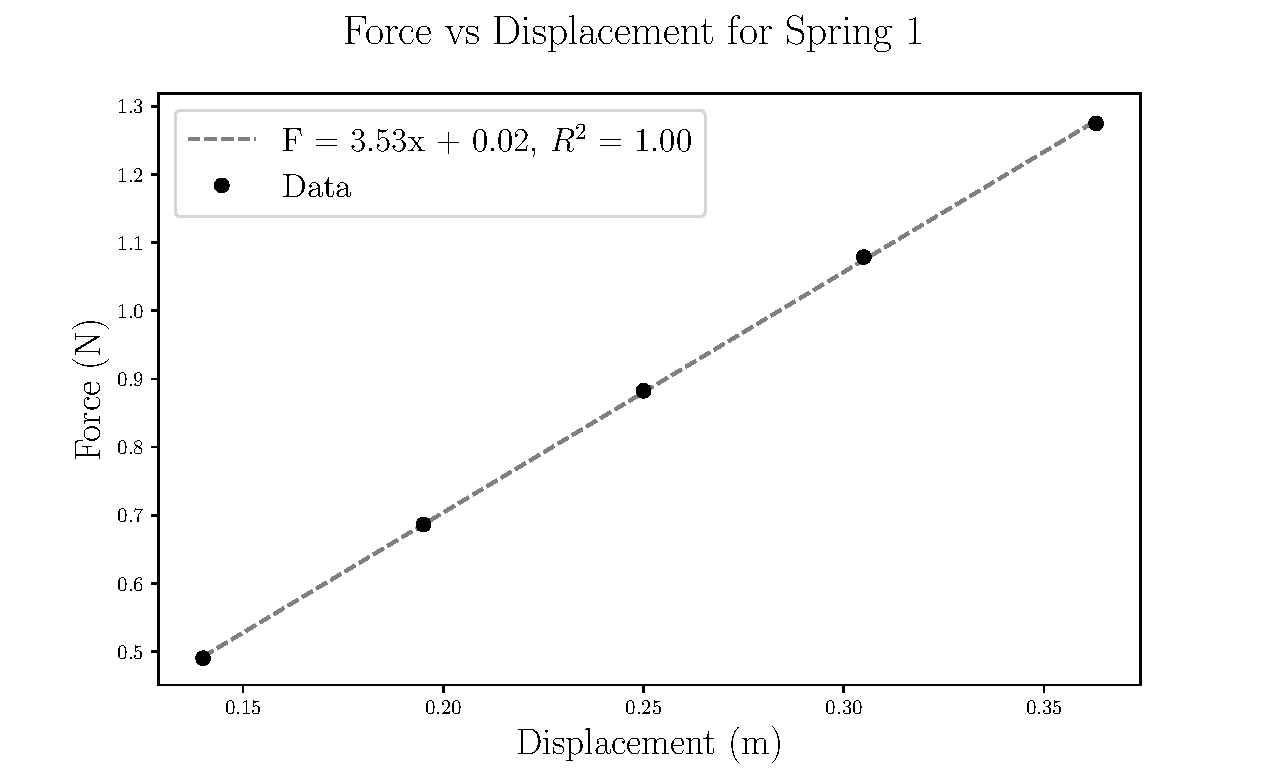
\includegraphics[scale=0.7]{spring_constant_1.pdf}
	\label{fig::spring1}
	\caption{Force (N) vs. Displacement (m) for spring 1 used in the harmonic oscillator system. Mass and, therefore, force was increased while the displacement of the spring from equilibrium was measured using a meter stick with an uncertainty of 0.05 cm; this uncertainty was not considered in calculation of the spring constant. The data was then linearly fit using Hooke's Law, $F = kx$, resulting in $k = 3.53 \pm 0.02$ N/m where the uncertainty was calculated from the fit's covariance matrix. Values obtained from Table \ref{tab::springTable}.}
\end{figure}

\begin{figure}[H]
    \centering
	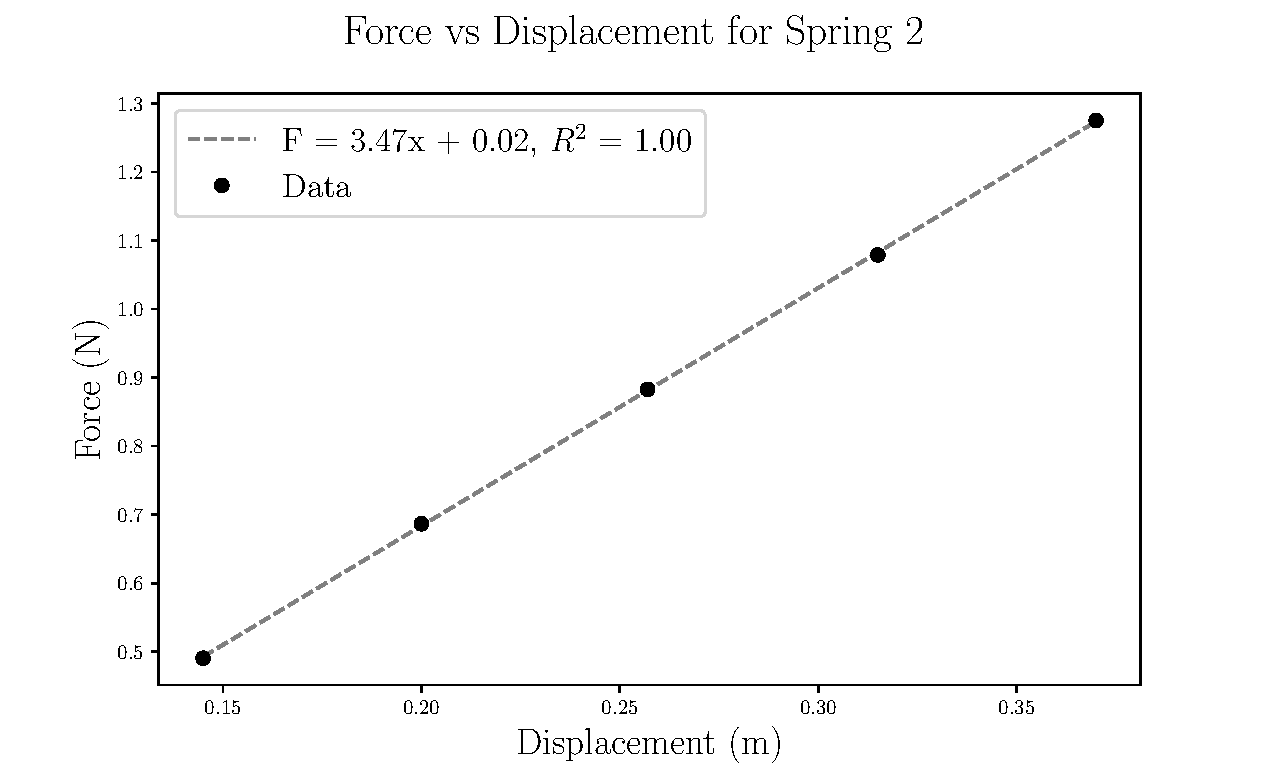
\includegraphics[scale=0.7]{spring_constant_2.pdf}
	\label{fig::spring2}
	\caption{Force (N) vs. Displacement (m) for spring 2 used in the harmonic oscillator system. Mass and, therefore, force was increased while the displacement of the spring from equilibrium was measured using a meter stick with an uncertainty of 0.05 cm; this uncertainty was not considered in calculation of the spring constant. The data was then linearly fit using Hooke's Law, $F = kx$, resulting in $k = 3.47 \pm 0.02$ N/m where the uncertainty was calculated from the fit's covariance matrix. Values obtained from Table \ref{tab::springTable}.}
\end{figure}

\begin{figure}[H]
    \centering
	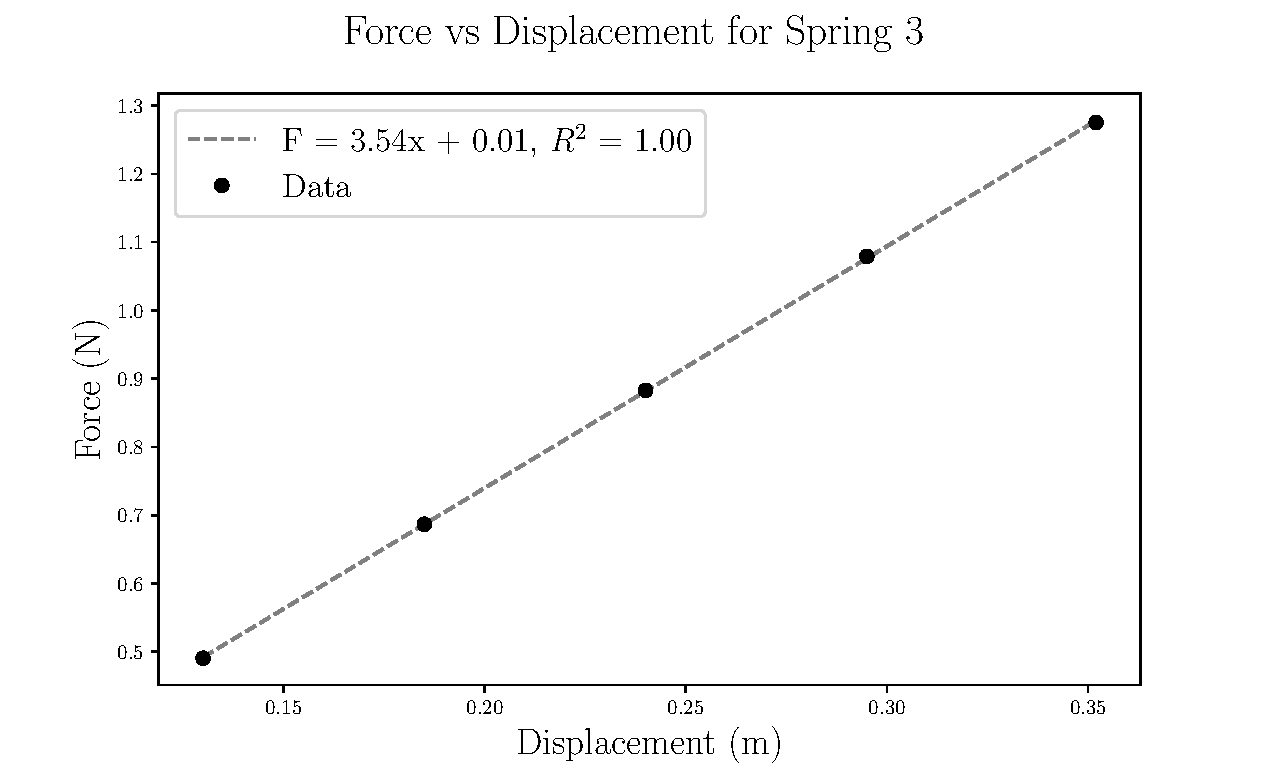
\includegraphics[scale=0.7]{spring_constant_3.pdf}
	\label{fig::spring3}
	\caption{Force (N) vs. Displacement (m) for spring 3 used in the harmonic oscillator system. Mass and, therefore, force was increased while the displacement of the spring from equilibrium was measured using a meter stick with an uncertainty of 0.05 cm; this uncertainty was not considered in calculation of the spring constant. The data was then linearly fit using Hooke's Law, $F = kx$, resulting in $k = 3.54 \pm 0.01$ N/m where the uncertainty was calculated from the fit's covariance matrix. Values obtained from Table \ref{tab::springTable}.}
\end{figure}

With the R$^2$ of each fit being 1.00 and each value having a low uncertainty, these values were deemed to be both accurate and precise. Furthermore, due to the similarity of the three spring constants, the average of the three, $k = 3.51 \pm 0.02$ N/m (assuming Gaussian) was used for the harmonic oscillator calculations.

\newpage
For the single air cart, forced, damped harmonic oscillator, the measured oscillation amplitude was plotted against the set driving frequency of the motor.

\begin{table}[H]
	\centering
	\begin{tabular}{ccc}
\toprule
 Driving frequency ($\pm 0.0005$ Hz) &  Oscillation amplitude ($\pm 0.05$ cm) \\
\midrule
                              0.410 &                                   0.3 \\
                              0.513 &                                   0.4 \\
                              0.607 &                                   0.5 \\
                              0.708 &                                   0.5 \\
                              0.805 &                                   0.9 \\
                              0.874 &                                   3.5 \\
                              0.883 &                                   4.5 \\
                              0.895 &                                  11.0 \\
                              0.911 &                                  11.5 \\
                              0.920 &                                  11.5 \\
                              0.924 &                                   5.5 \\
                              0.937 &                                   2.5 \\
                              0.949 &                                   1.5 \\
                              0.992 &                                   0.9 \\
                              1.016 &                                   0.6 \\
                              1.118 &                                   0.4 \\
                              1.216 &                                   0.3 \\
                              1.333 &                                   0.2 \\
\bottomrule
\end{tabular}

	\caption{The driving frequency (Hz) and oscillation amplitude (cm) for the single air cart, forced, damped harmonic oscillator with an air cart mass of $207.9 \pm 0.05$ g as measured by an electronic scale, with an uncertainty of $\pm 0.05$ g, and two springs with spring constants of $3.54 \pm 0.01$ N/m. The driving force was set manually on the motor interface, which had an uncertainty of $\pm 0.0005$ Hz, and the displacement was recorded using a ruler attached to the air track, which had an uncertainty of $\pm 0.05$ cm.}
	\label{tab::oscillationSingle}
\end{table}

\begin{figure}[H]
    \centering
	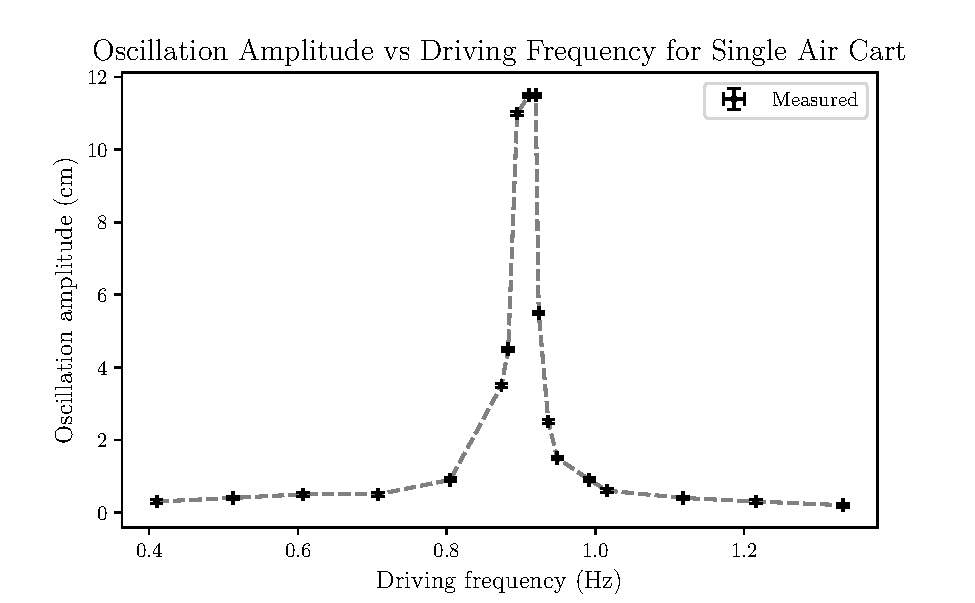
\includegraphics[scale=1]{oscillation_amplitude_vs_driving_frequency_single.pdf}
	\label{fig::resonanceSingle}
	\caption{Oscillation amplitude (cm) vs. driving frequency (Hz) for the single air cart, forced, damped harmonic oscillator with an air cart mass of $207.9 \pm 0.05$ g as measured by an electronic scale and two springs with spring constants of $3.54 \pm 0.01$ N/m. Values obtained from Table \ref{tab::oscillationSingle}.}
\end{figure}

With the resonance frequencies of a harmonic oscillator being the particular frequencies that result in a local oscillation amplitude maximum, the single resonance frequency of the single mass system was $0.920 \pm 0.0005$ Hz, due to it resulting in a maximum oscillation amplitude of $11.5 \pm 0.05$ cm. With the theoretical resonance frequency of the system being $0.926 \pm 0.002$ Hz, the experimental and theoretical values are not statistically equivalent; however, they are within three standard deviations of each other.

\begin{table}[H]
	\centering
	\begin{tabular}{cc}
\toprule
 Driving frequency ($\pm 0.0005$ Hz) &  Oscillation amplitude ($\pm 0.05$ cm) \\
\midrule
                               0.187 &                                    2.4 \\
                               0.269 &                                    1.2 \\
                               0.380 &                                    0.8 \\
                               0.486 &                                    0.8 \\
                               0.593 &                                    0.9 \\
                               0.696 &                                    1.2 \\
                               0.770 &                                    2.2 \\
                               0.795 &                                    2.3 \\
                               0.809 &                                    1.8 \\
                               0.820 &                                    2.1 \\
                               0.840 &                                    4.1 \\
                               0.855 &                                    5.2 \\
                               0.869 &                                   14.9 \\
                               0.885 &                                   12.2 \\
                               0.908 &                                    7.7 \\
                               0.924 &                                    4.2 \\
                               0.955 &                                    3.2 \\
                               0.973 &                                    2.2 \\
                               1.053 &                                    1.4 \\
                               1.205 &                                    0.8 \\
                               1.304 &                                    0.7 \\
\bottomrule
\end{tabular}

	\caption{The driving frequency (Hz) and oscillation amplitude (cm) for the single air cart, forced, damped harmonic oscillator with an increased air cart mass of $227.9 \pm 0.05$ g as measured by an electronic scale, with an uncertainty of $\pm 0.05$ cm, and two springs with spring constants of $3.54 \pm 0.01$ N/m. The driving force was set manually on the motor interface, which had an uncertainty of $\pm 0.0005$ Hz, and the displacement was recorded using a ruler attached to the air track, which had an uncertainty of $\pm 0.05$ cm.}
	\label{tab::oscillationSingleWeight}
\end{table}

\begin{figure}[H]
    \centering
	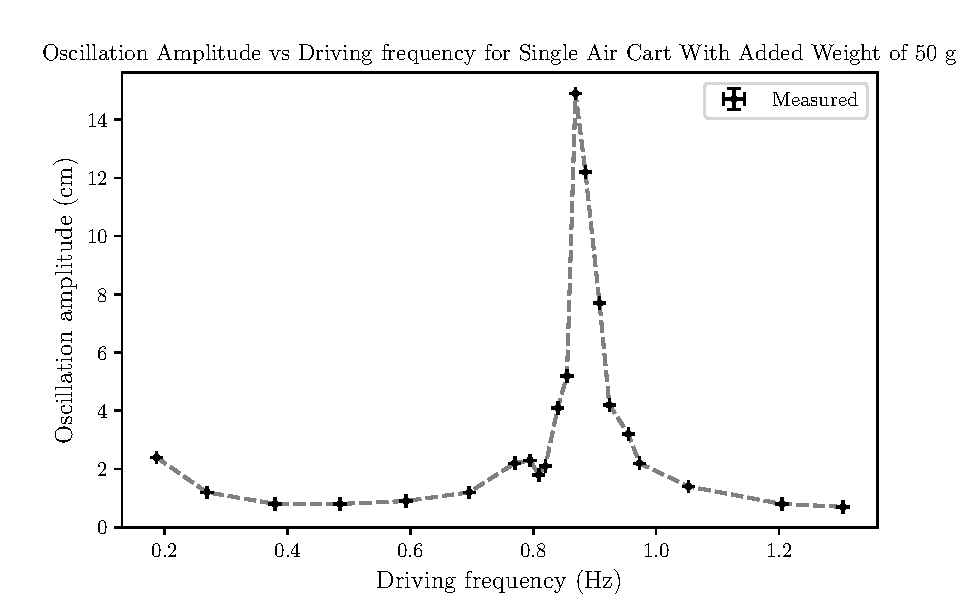
\includegraphics[scale=1]{oscillation_amplitude_vs_driving_frequency_single_weight.pdf}
	\label{fig::resonanceSingleWeight}
	\caption{Oscillation amplitude (cm) vs. driving frequency (Hz) for the single air cart, forced, damped harmonic oscillator with an increased air cart mass of $227.9 \pm 0.05$ g as measured by an electronic scale, with an uncertainty of $\pm 0.05$ g, and two springs with spring constants of $3.54 \pm 0.01$ N/m. Values obtained from Table \ref{tab::oscillationSingleWeight}.}
\end{figure}

Using the same method from the previous system, a resonance frequency of $0.869 \pm 0.0005$ Hz was obtained experimentally for the increased mass air cart. With the theoretical resonance frequency of the system being $0.884 \pm 0.002$ Hz, the experimental and theoretical values are not statistically equivalent.

\begin{table}[H]
	\centering
	\begin{tabular}{cc}
\toprule
 Driving frequency ($\pm 0.0005$ Hz) &  Oscillation amplitude ($\pm 0.05$ cm) \\
\midrule
                               0.186 &                                    0.4 \\
                               0.289 &                                    0.8 \\
                               0.388 &                                    0.4 \\
                               0.490 &                                    0.4 \\
                               0.584 &                                    2.2 \\
                               0.620 &                                    4.0 \\
                               0.636 &                                    5.5 \\
                               0.649 &                                   18.0 \\
                               0.658 &                                   16.5 \\
                               0.688 &                                    5.5 \\
                               0.708 &                                    2.0 \\
                               0.761 &                                    1.6 \\
                               0.815 &                                    1.0 \\
                               0.886 &                                    0.6 \\
                               0.928 &                                    1.5 \\
                               0.997 &                                    3.5 \\
                               1.055 &                                    4.2 \\
                               1.130 &                                    6.0 \\
                               1.217 &                                    3.5 \\
                               1.322 &                                    3.0 \\
                               1.401 &                                    2.2 \\
                               1.499 &                                    1.3 \\
                               1.602 &                                    0.7 \\
                               2.026 &                                    0.3 \\
                               2.512 &                                    0.2 \\
\bottomrule
\end{tabular}

	\caption{The driving frequency (Hz) and oscillation amplitude (cm) for the double air cart, forced harmonic oscillator with two air carts of masses $207.9 \pm 0.05$ g and $206.4 \pm 0.05$ g as measured by an electronic scale, with an uncertainty of $\pm 0.05$ g, and three springs with spring constants of $3.54 \pm 0.01$ N/m. The driving force was set manually on the motor interface, which had an uncertainty of $\pm 0.0005$ Hz, and the displacement was recorded using a ruler attached to the air track, which had an uncertainty of $\pm 0.05$ cm.}
	\label{tab::oscillationDouble}
\end{table}

\begin{figure}[H]
    \centering
	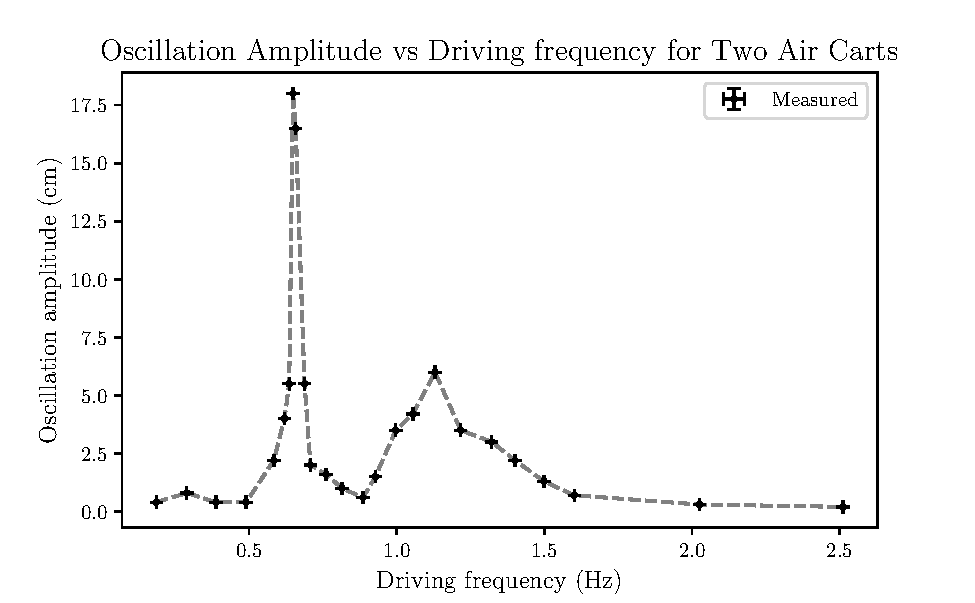
\includegraphics[scale=1]{oscillation_amplitude_vs_driving_frequency_double.pdf}
	\label{fig::resonanceDouble}
	\caption{Oscillation amplitude (cm) vs. driving frequency (Hz) for the double air cart, forced harmonic oscillator with two air carts of masses $207.9 \pm 0.05$ g and $206.4 \pm 0.05$ g as measured by an electronic scale, with an uncertainty of $\pm 0.05$ g, and three springs with spring constants of $3.54 \pm 0.01$ N/m. Values obtained from Table \ref{tab::oscillationDouble}.}
\end{figure}

For the double air cart system, as expected, we observed two resonance frequencies, represented by the two local maxima. In particular, the experimental \textit{slow} and \textit{fast} resonance frequencies were $0.649 \pm 0.0005$ Hz and $1.130 \pm 0.0005$ Hz, respectively. With the theoretical \textit{slow} and \textit{fast} resonance frequencies being $0.655 \pm 0.002$ Hz and $1.134 \pm 0.003$ Hz, respectively, neither of our experimental values were statistically equivalent to their theoretical expectations.












